%!TEX root = ../../Heun_Dale_Haney_A_dynamic_approach_to_input_output_modeling.tex
%%%%%%%%%%%%%%%%%%%%% chapter.tex %%%%%%%%%%%%%%%%%%%%%%%%%%%%%%%%%
%
% sample chapter
%
% Use this file as a template for your own input.
%
%%%%%%%%%%%%%%%%%%%%%%%% Springer-Verlag %%%%%%%%%%%%%%%%%%%%%%%%%%
%\motto{Use the template \emph{chapter.tex} to style the various elements of your chapter content.}
\motto{We try to measure what we value. 
We come to value what we measure.~\emph{\cite[p.~2]{Meadows:1998aa}}

\hfill---\emph{Donella Meadows}}

%%%%%%%%%%%%%%%%%%%%%%%%%%%%%%%%%
%%%%%%%%%% Value Flows %%%%%%%%%%
%%%%%%%%%%%%%%%%%%%%%%%%%%%%%%%%%
\chapter{Stocks and flows of economic value}
\label{chap:value} % Always give a unique label
% use \chaptermark{}
% to alter or adjust the chapter heading in the running head
\chaptermark{Value}
%%%%%%%%%%%%%%%%%%%%%%%%%%%%%%%%%
%%%%%%%%%%%%%%%%%%%%%%%%%%%%%%%%%
%%%%%%%%%%%%%%%%%%%%%%%%%%%%%%%%%




%% \abstract{Each chapter should be preceded by an abstract (10--15 lines long) that summarizes the content. The abstract will appear \textit{online} at \url{www.SpringerLink.com} and be available with unrestricted access. This allows unregistered users to read the abstract as a teaser for the complete chapter. As a general rule the abstracts will not appear in the printed version of your book unless it is the style of your particular book or that of the series to which your book belongs.\newline\indent
%% Please use the 'starred' version of the new Springer \texttt{abstract} command for typesetting the text of the online abstracts (cf. source file of this chapter template \texttt{abstract}) and include them with the source files of your manuscript. Use the plain \texttt{abstract} command if the abstract is also to appear in the printed version of the book.}

%% Use the template \emph{chapter.tex} together with the Springer document class SVMono (monograph-type books) or SVMult (edited books) to style the various elements of your chapter content in the Springer layout.


\abstract*{In this chapter, we develop techniques to account for flows of economic value
through economies.
We employ the prevailing subjective theory of value for our framework.
Value accounting equations were developed and applied to example
economies~A--C. % chktex 8
We noted the need for terms that describe creation and destruction
of value within economic sectors.
Finally, we explored value flows 
to and from the US auto economy
and found that, in contrast to material and energy, 
there is no lack of data on value flows.}


In Chapters~\ref{chap:direct_energy} and~\ref{chap:embodied_energy}, 
we noted that energy is the currency of thermodynamics,
and we developed accounting equations for flows and accumulation of 
direct ($\dot{E}$ and $\frac{\mathrm{d}E}{\mathrm{d}t}$) 
and embodied ($\dot{B}$ and $\frac{\mathrm{d}B}{\mathrm{d}t}$) 
energy through an economy.
In this chapter, we develop a framework for accounting
value flows~($\dot{X}$) through economies.
Accounting for flows and accumulation of economic value is 
routinely done in Systems of National Accounts,
however, this chapter demonstrates that such accounting
fits comfortably within the framework we have developed thus far
(Chapters~\ref{chap:materials}--\ref{chap:embodied_energy}).
Accounting flows of value within our framework is a necessary step along
the path to developing equations (in Chapter~\ref{chap:intensity}) 
that describe the energy intensity ($\varepsilon$) of intermediate
and final products within an economy.


%%%%%%%%%% Methodology %%%%%%%%%
\section{Subjective theory of value}
\label{sec:theory_of_value}

%%%%%%%%%%

We begin this chapter by explicitly stating what we mean by value. 
We follow the mainstream approach 
of using the market price at the time of an exchange
to determine the economic value of the flows of products (goods, services and capital). 
As materials and energy flow in one direction between sectors, 
currency flows in the opposite direction. 
The monetary flow is an easy and logical (though imperfect)
proxy for the value of the material and energy that exchanges hands from seller to buyer. 
Market transactions are easily documented, 
and the data 
to estimate the economic value of these flows 
is available in most countries.\cite{IIOA-Data}

Although the market price is readily available and conveys important information (such as
relative scarcity of the good and relative usefulness of the good to fulfill human wants), we note that market
price is \emph{subjective}.  
Value is based on the agreement of a mutally acceptable price 
by the human trading partners. 
The market price
is not a measure of any \emph{intrinsic}
value of the goods (e.g., for bio-diversity or ecosystem services). 
Market prices ignore the costs and benefits that accrue 
to other parties (externalities), 
including the impact of trade on the quality of human relations, 
just distribution of resources, 
or sustainable scale of the economy.\cite[p.~55]{Daly1997} 

The subjective theory of value,
while convenient and prevalent, does not
provide market participants with complete information, 
a particularly troubling fact in the age of resource depletion. 
(See Section~\ref{sec:change_needed}.)
The limitations of the subjective theory of value
have been a philosophical concern to 
economists, and others, since the beginning of economics.
Thoughout history, economists (particularly the classicals) 
and non-economists have searched for an invariant, objective, 
\emph{intrinsic} determinant of value, one that is not reliant 
solely on human wants at a particular point in time.%
	\footnote{
	Following the ecological economics literature, 
	we use the term \emph{intrinsic} in the sense of ``objective.'' 
	Costanza~\cite{Costanza:2004we} 
	notes that a better term would be objective, thereby avoiding
	moral overtones associated with the term intrinsic.
	} 
Adam Smith, Karl Marx, David Ricardo, and neo-Ricardian Piero Sraffa,
for example, have all proposed 
alternative determinants of value.  
Their proposed objective theories of value were based 
on identifying the primary input into production,
such as \emph{labor} (Marx) or \emph{land} (Malthus), 
and using that input as a numeraire, 
a way to measure value across the entire spectrum 
of goods and services in commensurate units.

More recently, some have proposed an \emph{energy} theory of value. 
Costanza~\cite{Costanza:2004we}, in particular, makes the case for energy 
as the only truly primary input into production 
and thus an, or rather \emph{the}, objective determinant of value. 
On a global scale, he notes, (solar) energy 
(including that which is stored in fossil fuels) is 
the only primary input into production:
everything else is an intermediate input. 
Thus, free energy input to production (accounting for all upstream energy)
could be the basis for an objective (intrinsic), 
energy theory of value.%
	\footnote{
	This line 
	of inquiry has yielded some interesting analysis of the amount 
	of solar energy required to run the economy. 
	See Chapter~\ref{chap:embodied_energy} for further discussion 
	of the concept of \emph{emergy}.
	}

Mainstream economics rejected the energy theory of value,
as well as all earlier alternative theories of value,
in favor of the subjective theory of value. 
However, as discussed in Section~\ref{sec:change_needed}, 
the information and signals provided by markets and prices 
may not be sufficient for national accounting in
the age of resource depletion. 
To paraphrase Herman Daly, 
national accounting focuses on measuring value-added, 
but it ignores ``that to which value is being added.'' \cite[p. 453]{Daly1995}
Ignoring the value provided by natural capital
distorts the measures of economic value provided by the subjective theory of value.
In particular, 
ignoring ``that to which value is being added'' 
tends to overestimate GDP. 
When easily accessible forms of energy 
(e.g., oil extracted from the Texas panhandle) 
are used up and more difficult locations must be tapped 
(e.g., Alaskan north slope or the Gulf of Mexico), 
the economy appears to grow.
The ``value-added'' by human and manufactured capital increases 
as humans must do more work to extract increasingly marginal 
energy resources. 
However, what is actually happening is that the stock 
of natural resources is diminishing in both quantity and quality, 
and the drawdown of natural capital is (mis)measured by GDP as 
an increase in income.\cite[pp.~66~and~75]{Daly1997}

As discussed in Chapter~\ref{chap:intro}, 
when the level of the stock of ``that to which value is added'' 
(natural capital) declines, 
the economy begins to reach binding material and energy constraints, 
and economic growth suffers. 
Thus, identifying the right economic 
scale---the rate at which materials are put through the 
economy---becomes an optimization problem. 
If the material throughput rate is too small, 
economies don't provide enough goods and services for society.
If the material throughput rate is too high, 
the biosphere cannot replenish natural resources fast enough and
binding constraints are reached with dire economic consequences.
Unfortunately, this is an optimization 
problem that the market alone cannot solve. 

Despite the considerable drawbacks to the subjective theory of value, 
using market transactions to confer economic value
on flows of energy and material goods is widely accepted and understood.
Better measures of value are difficult to implement. 
Thus, in the development of our framework, 
we use market prices at the time of transaction to determine the value of 
material and energy flows.
However, we do so for pragmatic, rather than philosophical, reasons.

That being said, we also believe that our framework demonstrates the  
urgent need for additional valuation methods to be used
alongside market prices to provide the information
needed for national accounting in the age of resource depletion. 
The UN System of Environmental-Economic Accounting (SEEA)%
	\footnote{
	As of this printing, 
	the System of Environmental-Economic Accounting (SEEA)~\cite{UNSEEA2014}
	is in its third edition, having been thouroughly reviewed and revised 
	by a global consultation process. 
	The SEEA contains internationally agreed-upon standards for quantifying the 
	value of flows of material and energy between the economy and the biosphere. 
	SEEA is a system that is designed to 
	work hand in hand with the System of National Accounts (SNA), 
	the international standard for measuring economic value creation consistently across nations,
	and several OECD member states
	currently use the SEEA alongside their national accounting.
	} 
provides rigorous methodology to estimate the value 
of material and energy flows between the biosphere and the economy.
(See Figure~\ref{fig:basic_value_with_biosphere_flows}.)
Such a system should be used consistently by all
nations to estimate the value of these flows, 
as depicted in the accounting framework below.
Without SEEA, or something similar,%
	\footnote{
	As described in the Prologue, the US BEA developed
	its analogous methodolgy in the early 1990s, 
	the Integrated Environmental Economic System of Accounts (IEESA), 
	but has been politically hamstrung for
	over 20 years from publishing the data.
	}
these flows cannot be valued. 
Thus, those flows are conspicuously 
absent from the model for the flow of economic value presented in the next section.
(See, e.g., Figure~\ref{fig:basic_value}.)

\begin{figure}[ht!]
\centering\
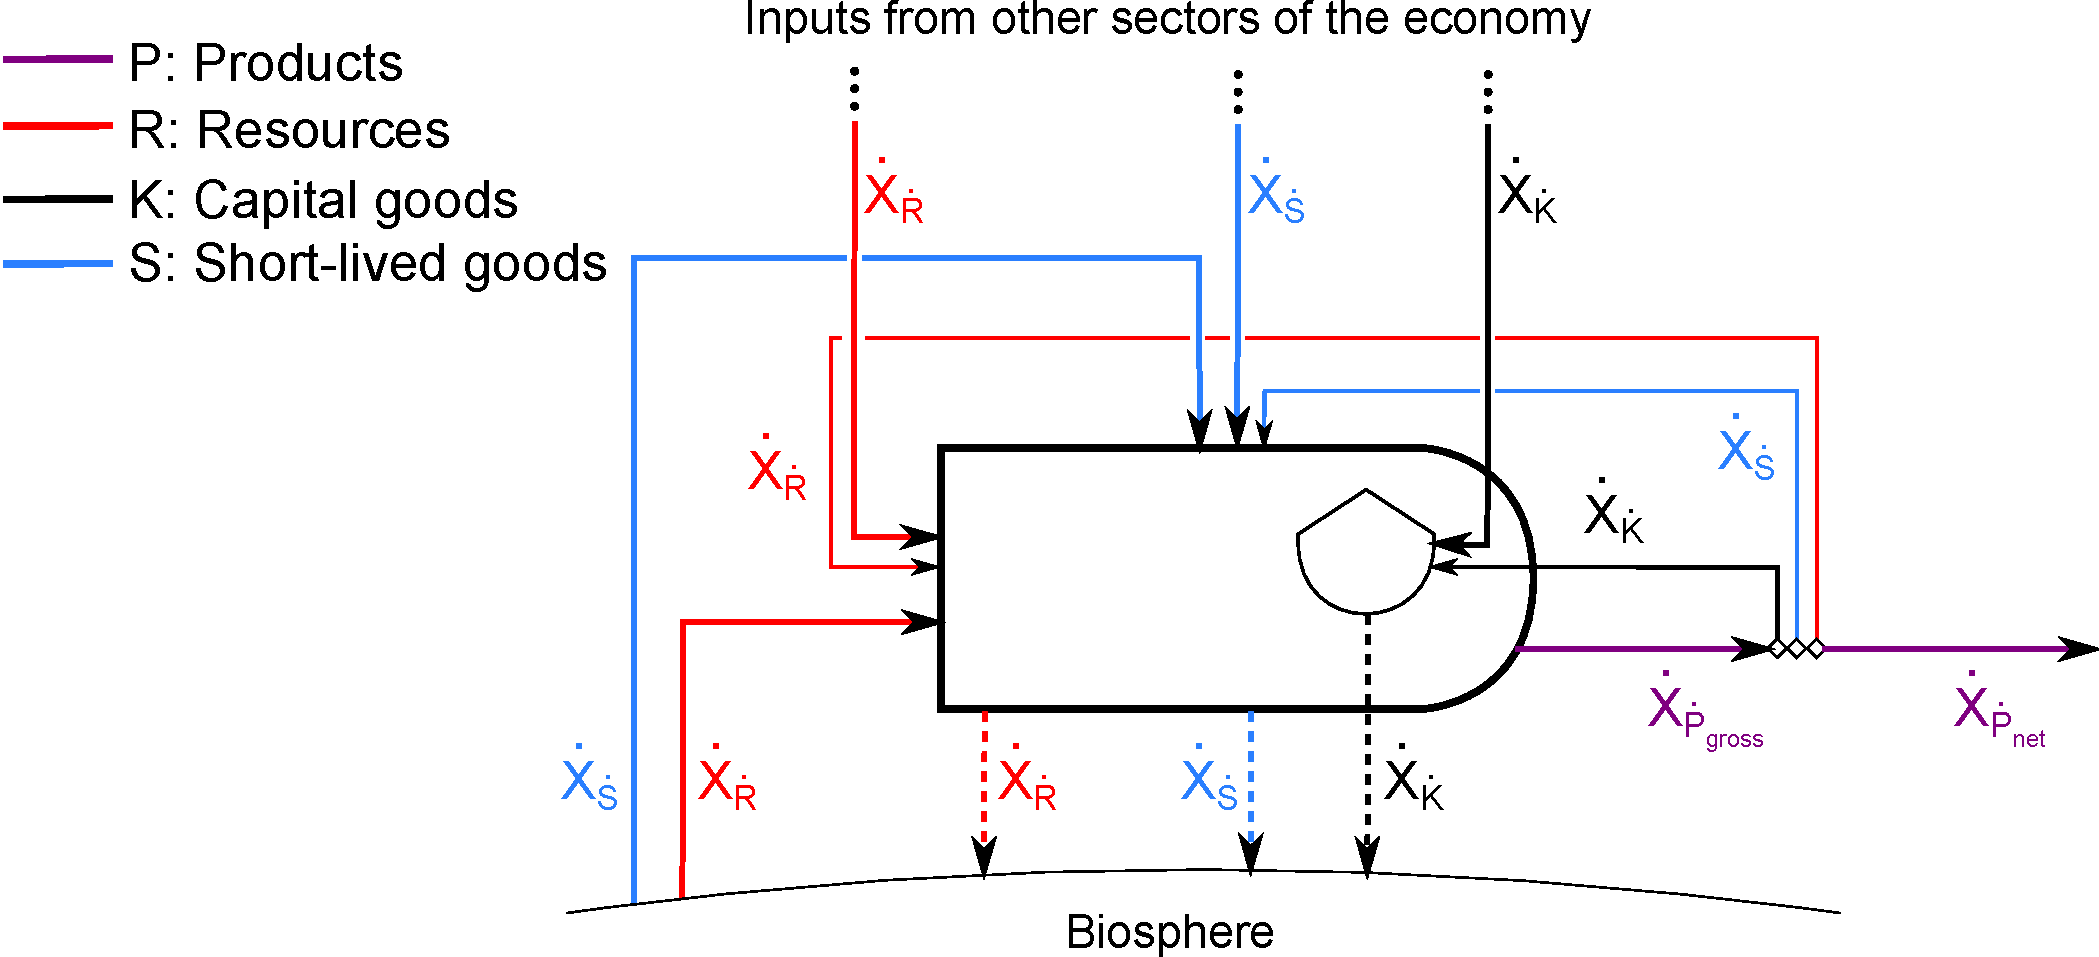
\includegraphics[width=0.8\linewidth]{Part_2/Chapter_Values/images/PERKS_basic_unit_value_with_biosphere_flows.pdf}
\caption[Aggregated flows of value for a single sector including flows to and from the biosphere]{Aggregated flows of value for a single sector, including flows to and from the biosphere.}
\label{fig:basic_value_with_biosphere_flows}
\end{figure}


%******** Value methodology *****
\section{Methodology}
\label{sec:Value_Methodology}
%%%

Because the basic unit of analysis in our framework is the economic sector, 
flows of value within the economy are based on the prices  
from inter-sectoral market transactions. 
The flows of value that accompany material and energy flows in and out 
of one sector in an economy are depicted in Figure~\ref{fig:basic_value}. 
The solid lines represent flows of economic value whose direction
is the same as the flow of material and energy.
The dashed lines represent the equal and opposite
flows of currency used to pay for the material and energy.%
	\footnote{
	Because the currency lines clutter the diagram,
	we will omit currency flows from all following diagrams in this chapter.
	}
The price diamonds (also seen in Figures~\ref{fig:perp_motion_1}--\ref{fig:metabolic_economy})
indicate that the economic value of material and energy flows is
set by agreement between buyers and sellers, the subjective theory of value.

\begin{figure}[!ht]
\centering
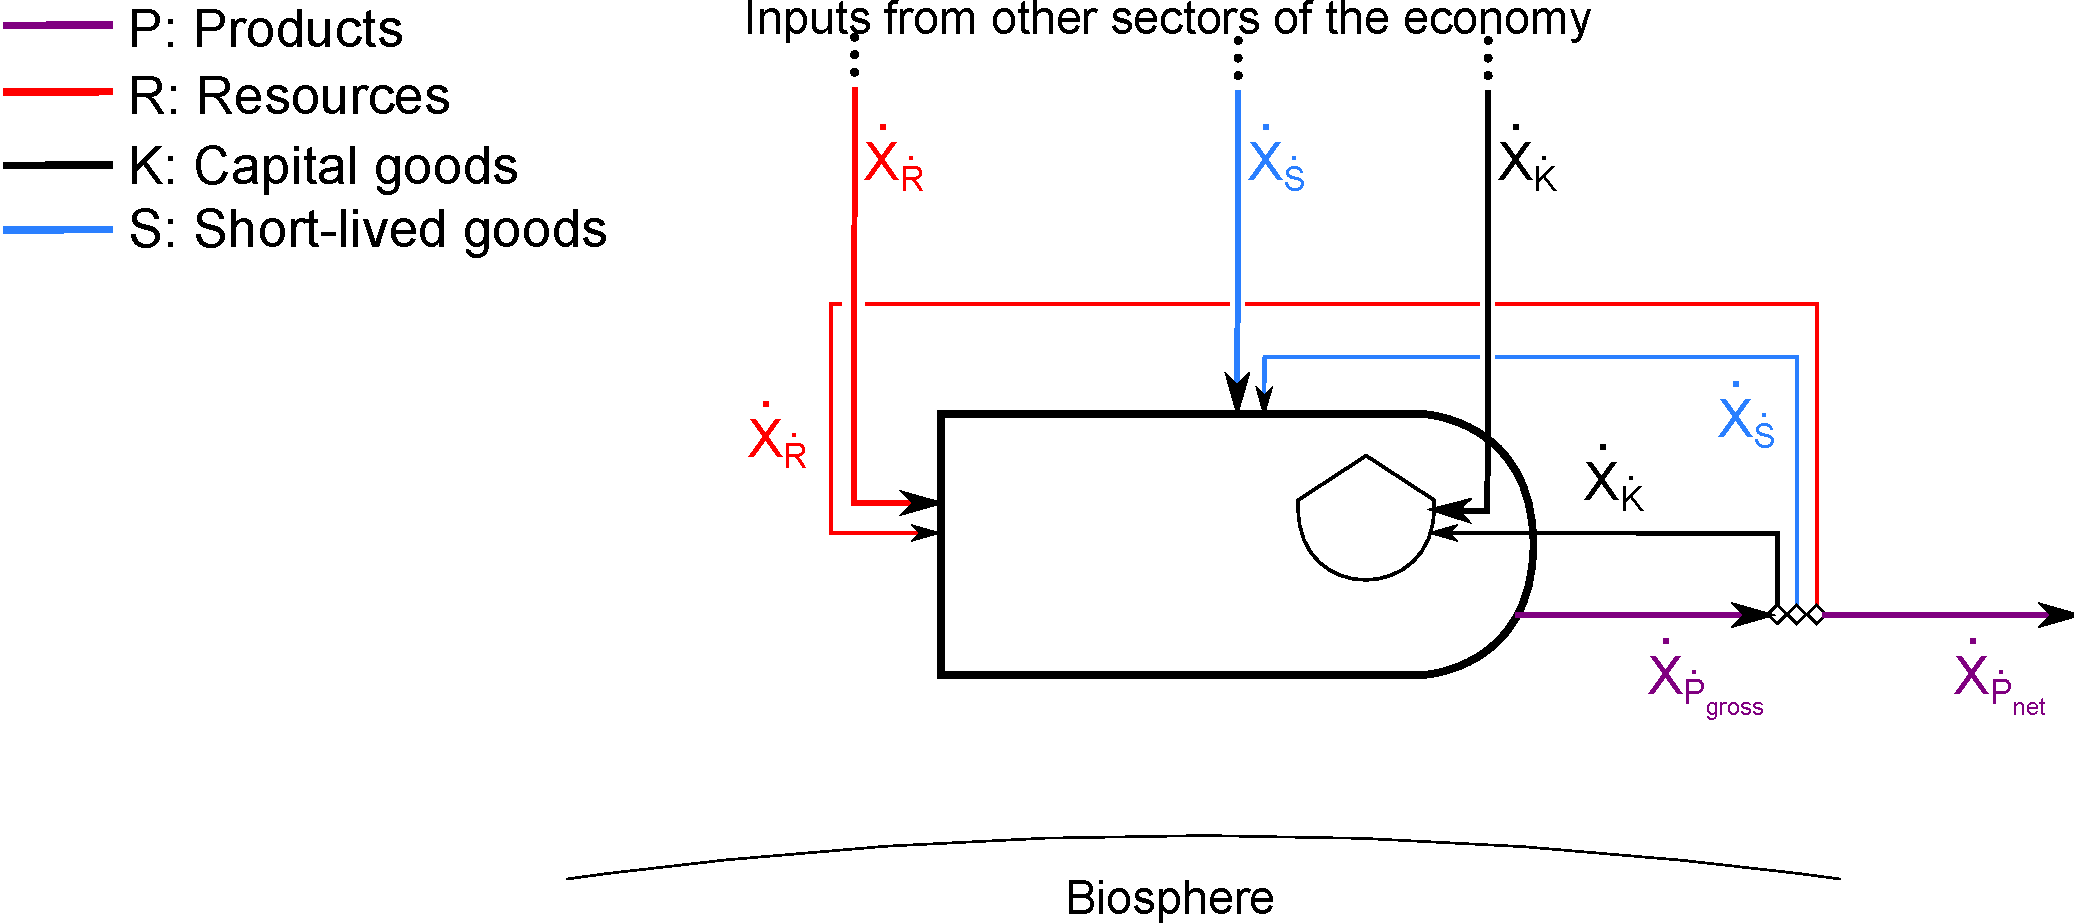
\includegraphics[width=\linewidth]{Part_2/Chapter_Values/images/PERKS_basic_unit_value_all.pdf}
\caption[Flows of value for a single sector]{Flows of economic value ($\dot{X}$) 
for a single sector. 
The economic value flows are associated with each of the different 
material and energy flows outlined in previous chapters. 
The dashed lines represent the equal and opposite flows of the 
currency used to pay for the 
material and energy.}
\label{fig:basic_value} 
\end{figure}

As mentioned in the discussion of the subjective theory of value 
in Section~\ref{sec:theory_of_value}, national accounting focuses on
measuring value-added. 
We denote creation and destruction of value within a sector 
using the notion of ``source'' and ``sink.''
In Figure~\ref{fig:basic_value_aggregated}, the open circle, 
``source,'' inside the economic sector represents the value-added,
that is, the value that is created by the economic processes within that sector. 
Flows of economic value from a value-source are denoted $\dot{X}_{gen}$. 
Similarly, filled circles represent the value ``sinks''  where value is destroyed 
by economic processes or natural disasters. 
Flows of economic value into a value-sink are denoted $\dot{X}_{dest}$. 
Although we do not define 
the value creation and destruction processes any further (mathematically), 
we discuss what is meant by the
underlying processes in Section~\ref{sec:value_generation}.

\begin{figure}[!ht]
\centering
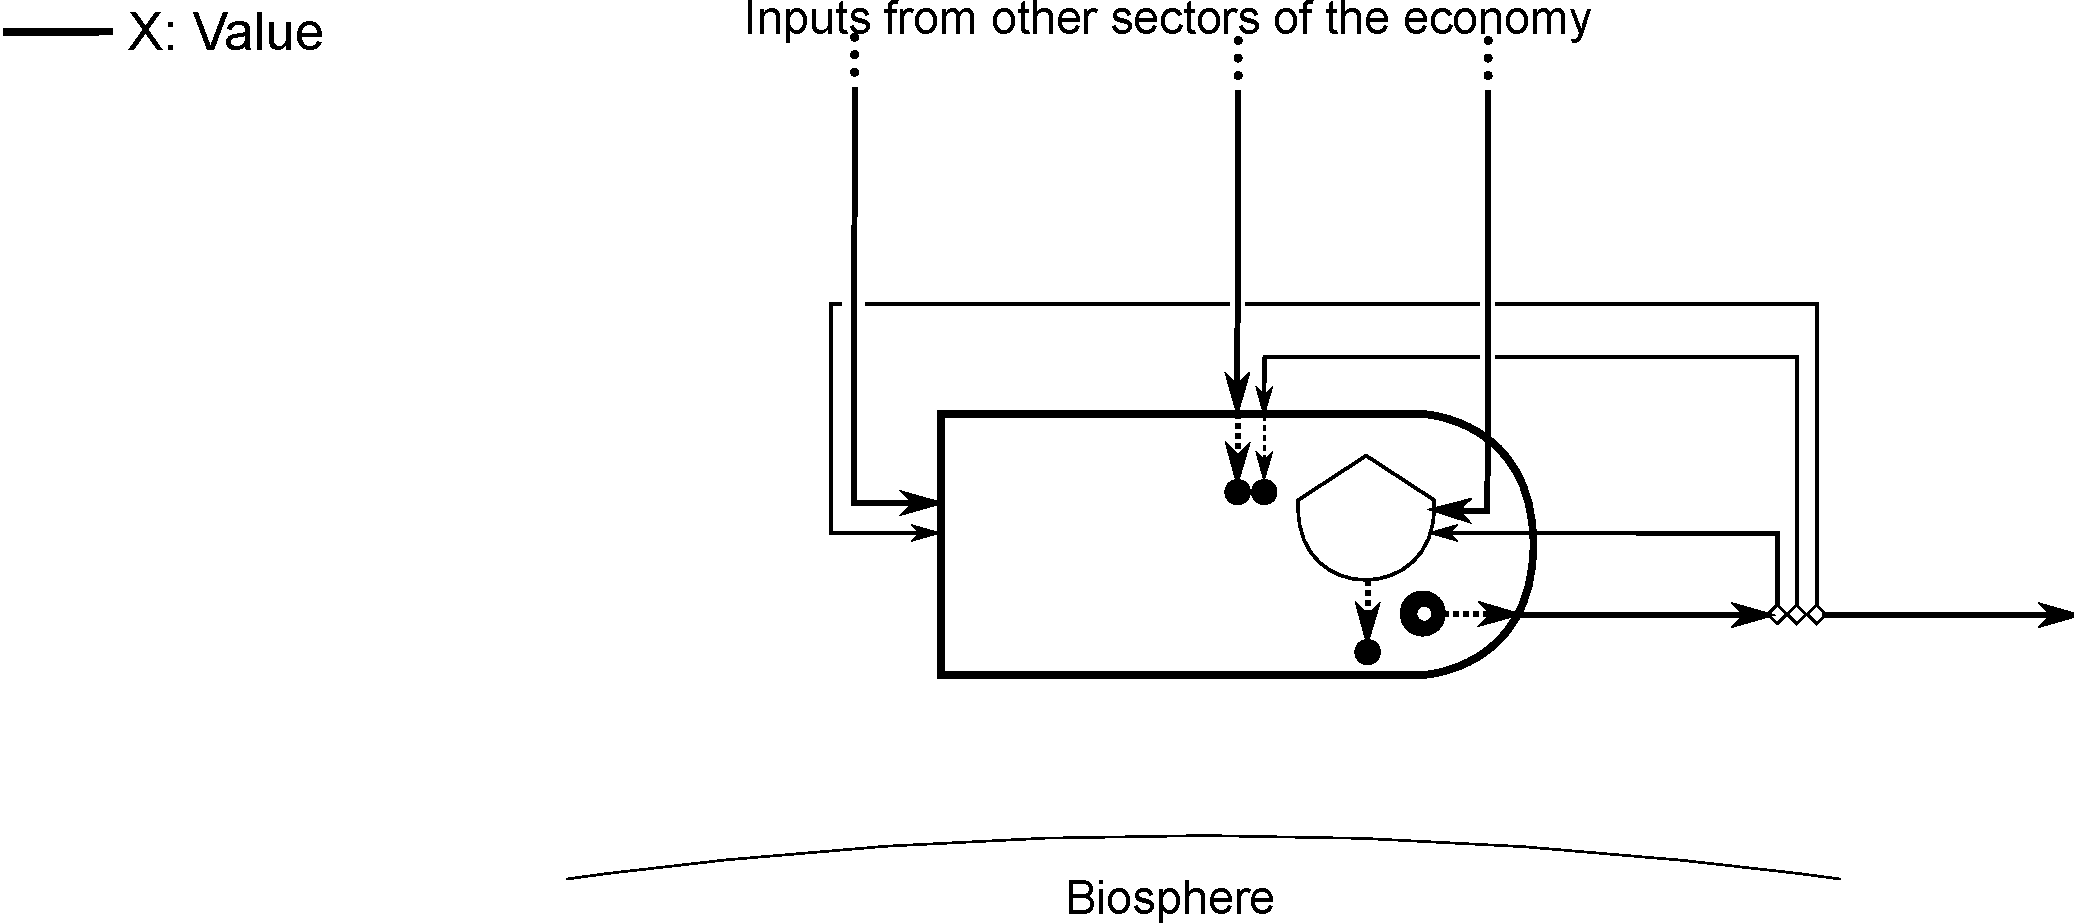
\includegraphics[width=\linewidth]{Part_2/Chapter_Values/images/PERKS_basic_unit_value.pdf}
\caption[Aggregated flows of value for a single sector]{Aggregated flows of value ($\dot{X}$) 
for a single sector. 
Distinction is made between value flows that 
enter the sector and are accumulated (i.e.\ capital goods) 
and value flows that are not accumulated. 
Within the sector there is destruction of value $\dot{X}_{dest}$, 
represented by the downward arrow flowing 
into the filled-circle sinks and generation of value, 
represented by the arrow flowing out of an open-circle source.}
\label{fig:basic_value_aggregated} 
\end{figure}


%%%%%%%%%% Example A: single-sector economy %%%%%%%%%%
\section{Example~A: single-sector economy} % chktex 13
\label{sec:value_example_A}
%%%%%%%%%%

Figure~\ref{fig:A_value} shows flows of value in the single-sector economy.
Following typical assumptions in economic modeling, 
the economy is \emph{completely isolated} from the biosphere
in terms of both material inputs and wastes.
In other words, the value flows of an economy are \emph{independent from}
material inputs and wastes.
Value flows are independent from material inputs,
because raw materials have no economic value 
until they have been removed from the biosphere by an extraction industry.
Value flows are independent from wastes,
because wastes, by definition, have no economic value 
upon leaving the economy.

\begin{landscape}
\begin{figure}[!ht]
\centering
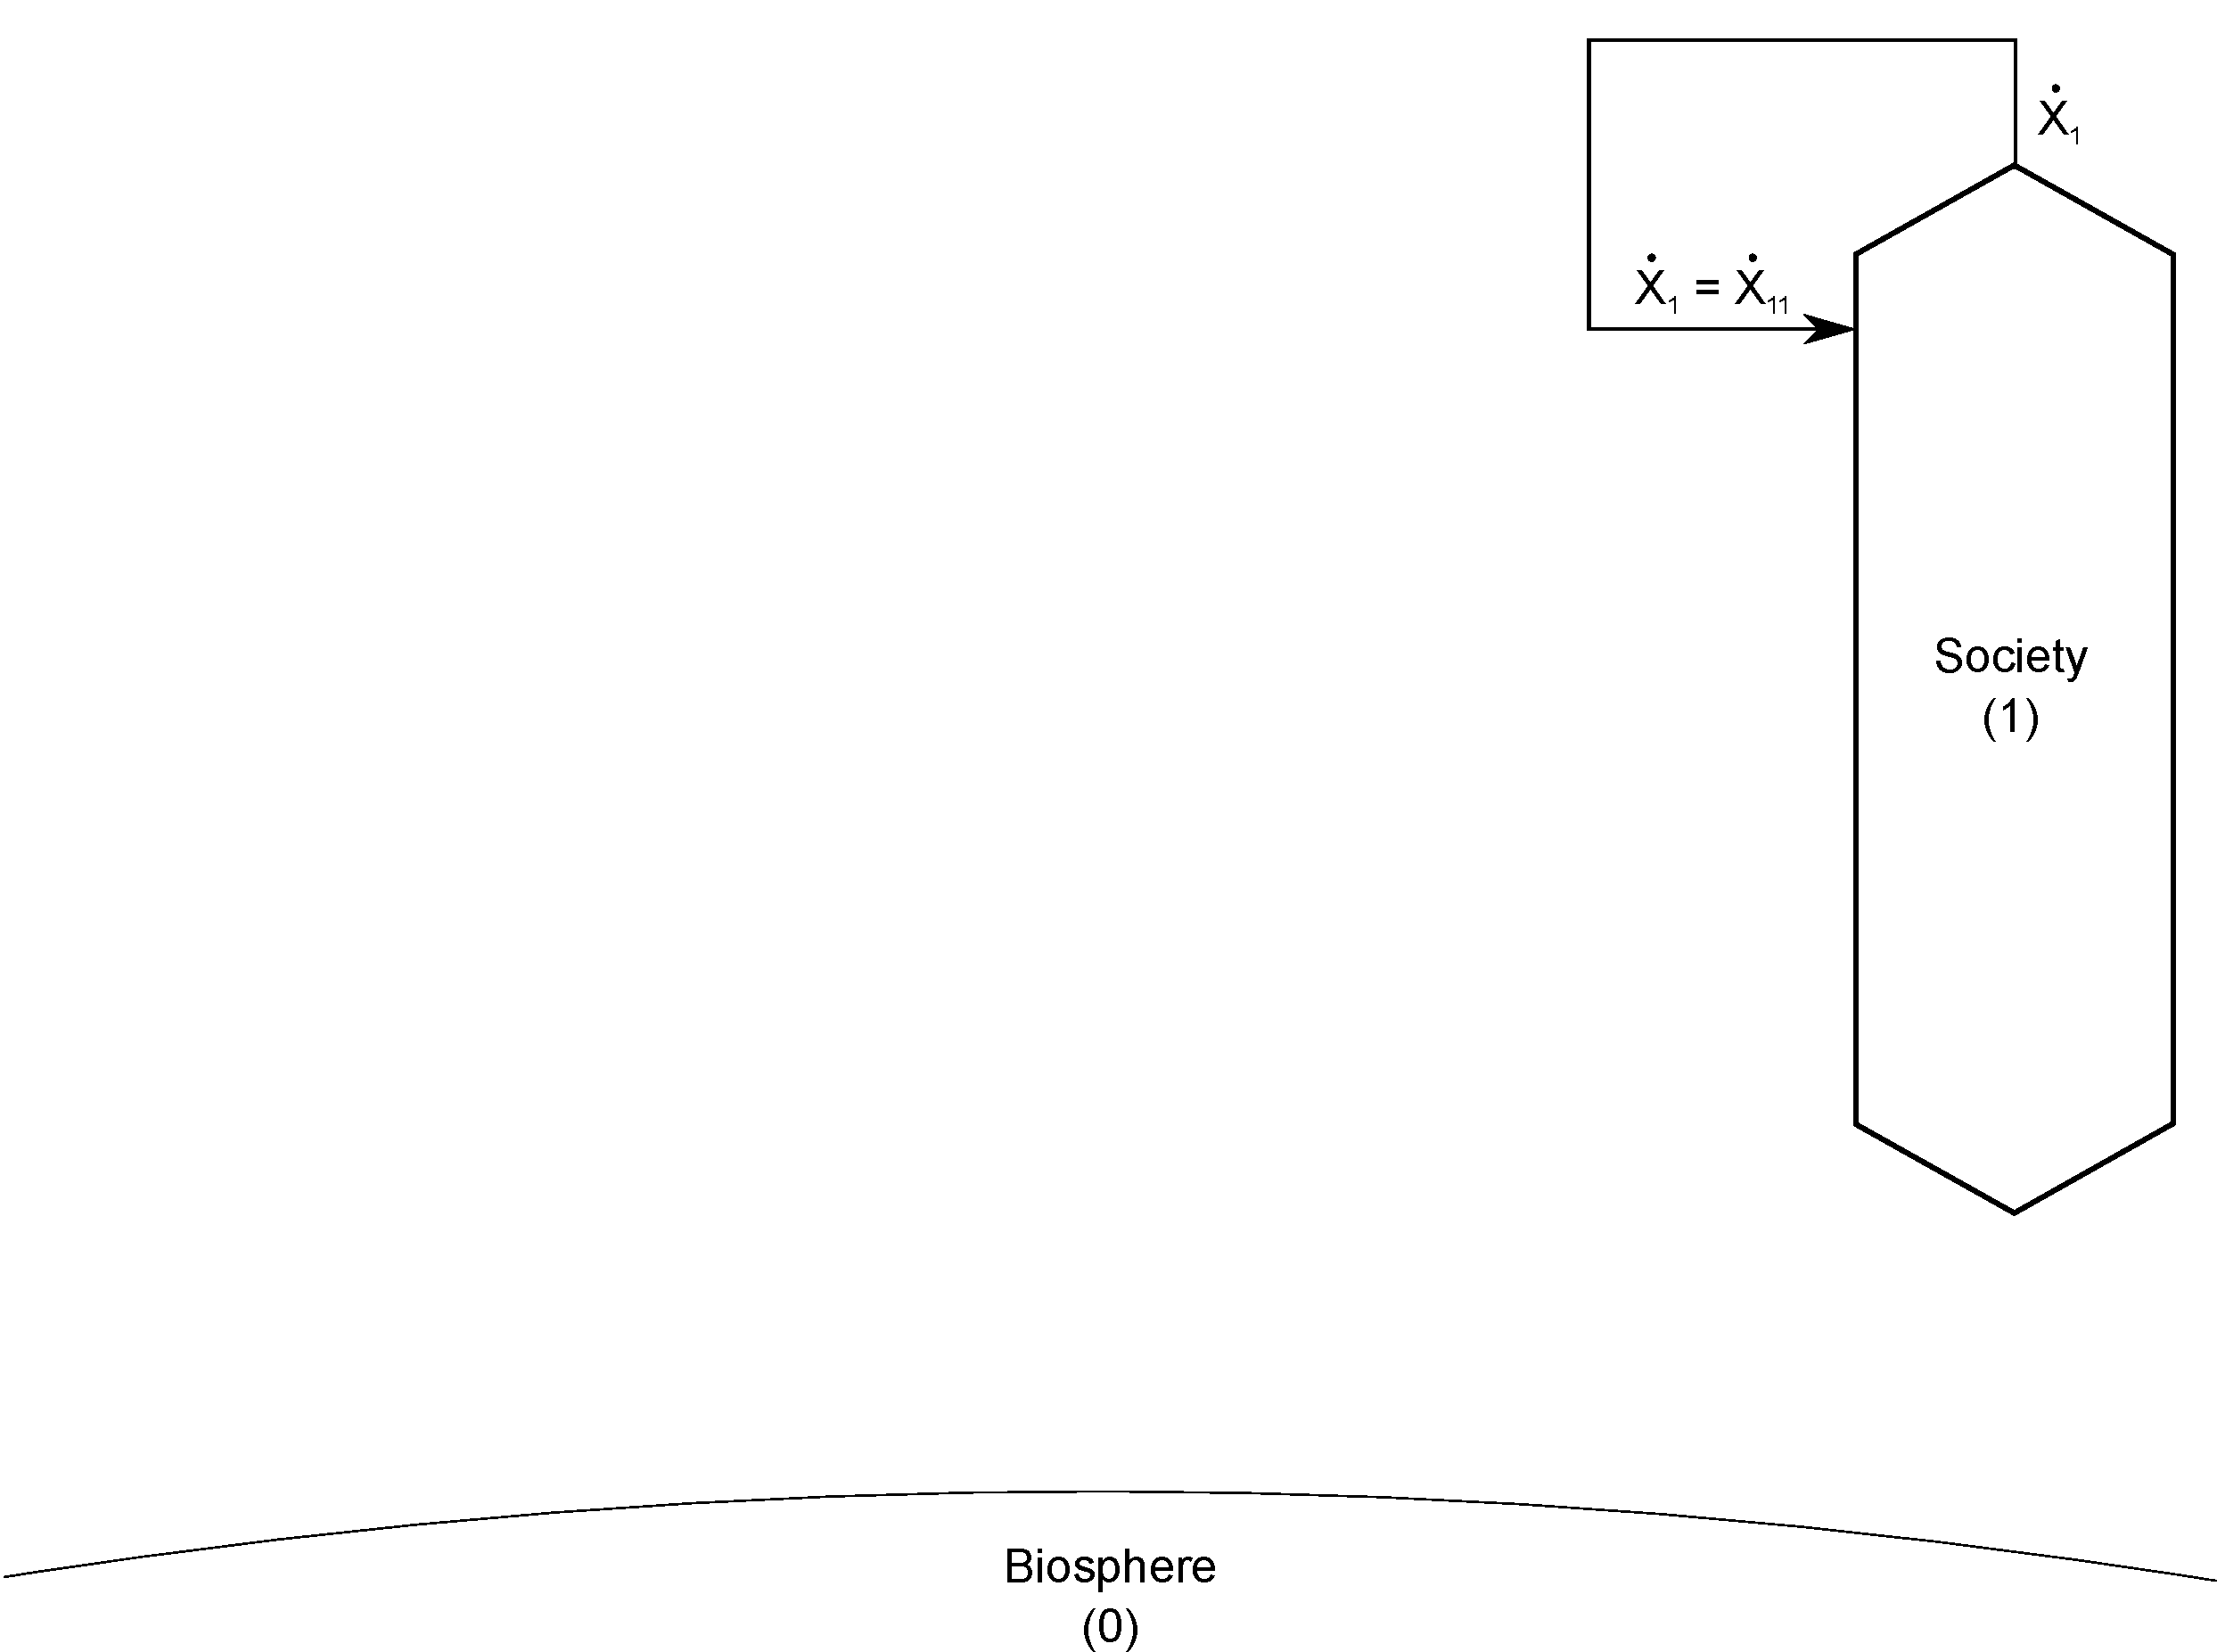
\includegraphics[width=0.8\linewidth]{Part_2/Chapter_Values/images/1_sector_value.pdf}
\caption[Flows of value for a one-sector economy]{Flows of value ($\dot{X}$) for a one-sector economy.}
\label{fig:A_value} 
\end{figure}
\end{landscape}

The contrast between the biophysical picture
(as represented in Figures~\ref{fig:A_materials}~and~\ref{fig:A_energy})
on the one hand, 
and the conventional viewpoint of economics
(as represented in Figure~\ref{fig:A_value}) 
on the other, is striking.  
The biophysical picture of material and energy flows in 
Figures~\ref{fig:A_materials} and~\ref{fig:A_energy} 
emphasizes interaction with and dependence upon the biosphere 
that is not reflected in the typical economic model of 
value flows depicted in Figure~\ref{fig:A_value}.
As discussed in Section~\ref{sec:theory_of_value},
the isolation of the value flows from the biosphere is a consequence
of the subjective theory of value
that underpins modern economics.
The biosphere is akin to a third party with no voice 
in determining the value of a transaction:
it is neither buyer nor seller. 

Equation~\ref{eq:A_X_acct_1} describes the accumulation 
of value~($X$) in Society~(1).
%
\begin{equation} \label{eq:A_X_acct_1}
	\frac{\mathrm{d}X_{1}}{\mathrm{d}t} 
	= \dot{X}_{11} 
	- \dot{X}_{1}
	+ \dot{X}_{gen,1}
	- \dot{X}_{dest,1}.
\end{equation}
%
The following subsections discuss the terms in Equation~\ref{eq:A_X_acct_1}.


%+++++++++ Example A: Economic Transactions ++++++++++
\subsection[Economic transactions]{Economic transactions ($\dot{X}_{11}$ and $\dot{X}_{1}$)}
%+++++++++

The returning arrow in Figure~\ref{fig:A_value} 
represents transactions between 
%
\begin{itemize}

	\item{buyers (who receive things of value, $\dot{X}_{11}$,
	in exchange for currency) and}

	\item{sellers (who give up things of value, $\dot{X}_{1}$,
	in exchange for currency).}

\end{itemize}
%
It is interesting to note that when a good is sold for more
than the producer paid for its inputs, 
the seller has created value and sold it into the economy. 
As a consequence, the seller's stock of currency grows,
providing the seller with an increased level of claim 
on value in the economy.

The subjective theory of value~(Section~\ref{sec:theory_of_value})
posits that buyers and sellers agree on value at the 
time of the transaction.
Thus, $\dot{X}_{1} = \dot{X}_{11}$, and Equation~\ref{eq:A_X_acct_1}
simplifies to
%
\begin{equation} \label{eq:A_X_acct_2}	
	\frac{\mathrm{d}X_{1}}{\mathrm{d}t}	
	= \dot{X}_{gen,1}
	- \dot{X}_{dest,1},
\end{equation}
%
indicating that value accumulates in the economy
$\left( \frac{\mathrm{d}X_{1}}{\mathrm{d}t} \right)$
due to value generation ($\dot{X}_{gen,1}$) 
and destruction ($\dot{X}_{dest,1}$) processes only.


%+++++++++ Example A: value generation ++++++++++
\subsection[Value generation]{Value generation ($\dot{X}_{gen}$)}
\label{sec:value_generation}
%+++++++++

\noindent In Equation~\ref{eq:A_X_acct_1}, 
the value generation term ($\dot{X}_{gen}$) is akin to growing apples.
The term $\dot{X}_{gen}$ is accounted as ``value added'' to an industry in national accounts.
It is calculated as the difference between gross economic output of the industry
and the cost of its intermediate inputs.\cite{BEAVA}  
A simple way to think of value added is
the increase in value of the raw materials from the work performed 
on them by workers and manufactured capital.


Much
of the 
value added that is attributed to the manufacturing
process was actually value provided by 
natural capital, at  no  
monetary cost to producers. For example, in Section~\ref{sec:Materials_Methodology}, the
apples that are produced would be counted
in national accounting as value added by capital 
and labor, when in reality, the value is provided
by the biosphere and natural capital, including:
%
\begin{itemize}
	
	\item{the flow of solar energy
	into the economy, directly as in the case
	of growing apples, and indirectly as energy embodied
	in fossil fuels}
	
	\item{the extraction of resources (e.g., water, minerals, and
	fossil fuels) or any other unpriced goods from the biosphere, and}
	
	\item{the exploitation of the unpriced waste assimilation capacity of the biosphere.}
	
\end{itemize}
%
The subjective theory of value indicates that 
there is no economic value associated with these ``transactions,'' 
because no currency is exchanged. 

The above factors indicate that the process of value generation
has both direct and indirect impacts on the biosphere.
The direct impacts are obvious: 
extraction of non-renewable resources from the biosphere, 
at rates greater than their natural accretion,
represents unsustainable overuse of natural capital.
The indirect impacts are less obvious: 
the value generated by these transactions can lead to increased wealth,
leading to increased demand rates for goods and services, 
whose production requires ever-increasing rates 
of unsustainable natural resource extraction.


%+++++++++ Example A: value destruction ++++++++++
\subsection[Value destruction]{Value destruction ($\dot{X}_{dest}$)}
%+++++++++

In Equation~\ref{eq:A_X_acct_1}, 
the value destruction term ($\dot{X}_{dest}$)
is akin to consuming apples: 
value is destroyed by a process that consumes, 
or otherwise renders unusable, 
previously-valuable things in the economy
(see Section~\ref{sec:Materials_Methodology}).
The factors that lead to value destruction
($\dot{X}_{dest}$) include:
%
\begin{itemize}

	\item{depreciation, usually associated with disposal of 
	materials and equipment to the biosphere at end of life and}

	\item{natural disasters, such as hurricanes and typhoons,
	that destroy equipment and property.}

\end{itemize}
%
$\dot{X}_{dest}$ is accounted as depreciation, 
or ``consumpton of fixed capital,'' % chktex 38
to an industry in the national accounts. 
It is a monetary estimate of the physical effects on assets from 
``wear and tear, obsolescence, accidental damage,
and aging.''~\cite{katz2008} 


%+++++++++ Example A: GDP and Stock of Value ++++++++++
\subsection{GDP}
%+++++++++

If Society (1) in Figure~\ref{fig:A_value} represents 
the economy of an entire country, 
$\dot{X}_{1}$ is its gross domestic product (GDP)
in units of \$/year. 
Alghough GDP is often considered a stock, it is not. 
It is a flow. 
$X_{1}$ is a stock, akin to monetary wealth. 
However, $X_{1}$ is a very
narrow definition of wealth
that neglects the value of natural resources, 
the value of social captial, and any
other ``wealth'' that cannot be exchanged for money. 


%%%%%%%%%% Example B: two-sector economy %%%%%%%%%%
\section{Example~B: two-sector economy} % chktex 13
%%%%%%%%%%

Figure~\ref{fig:B_value} shows flows of value ($\dot{X}$) 
within a two-sector economy. 
Again, we note the isloation of the economy from the biosphere.

\begin{landscape}
\begin{figure}[!ht]
\centering
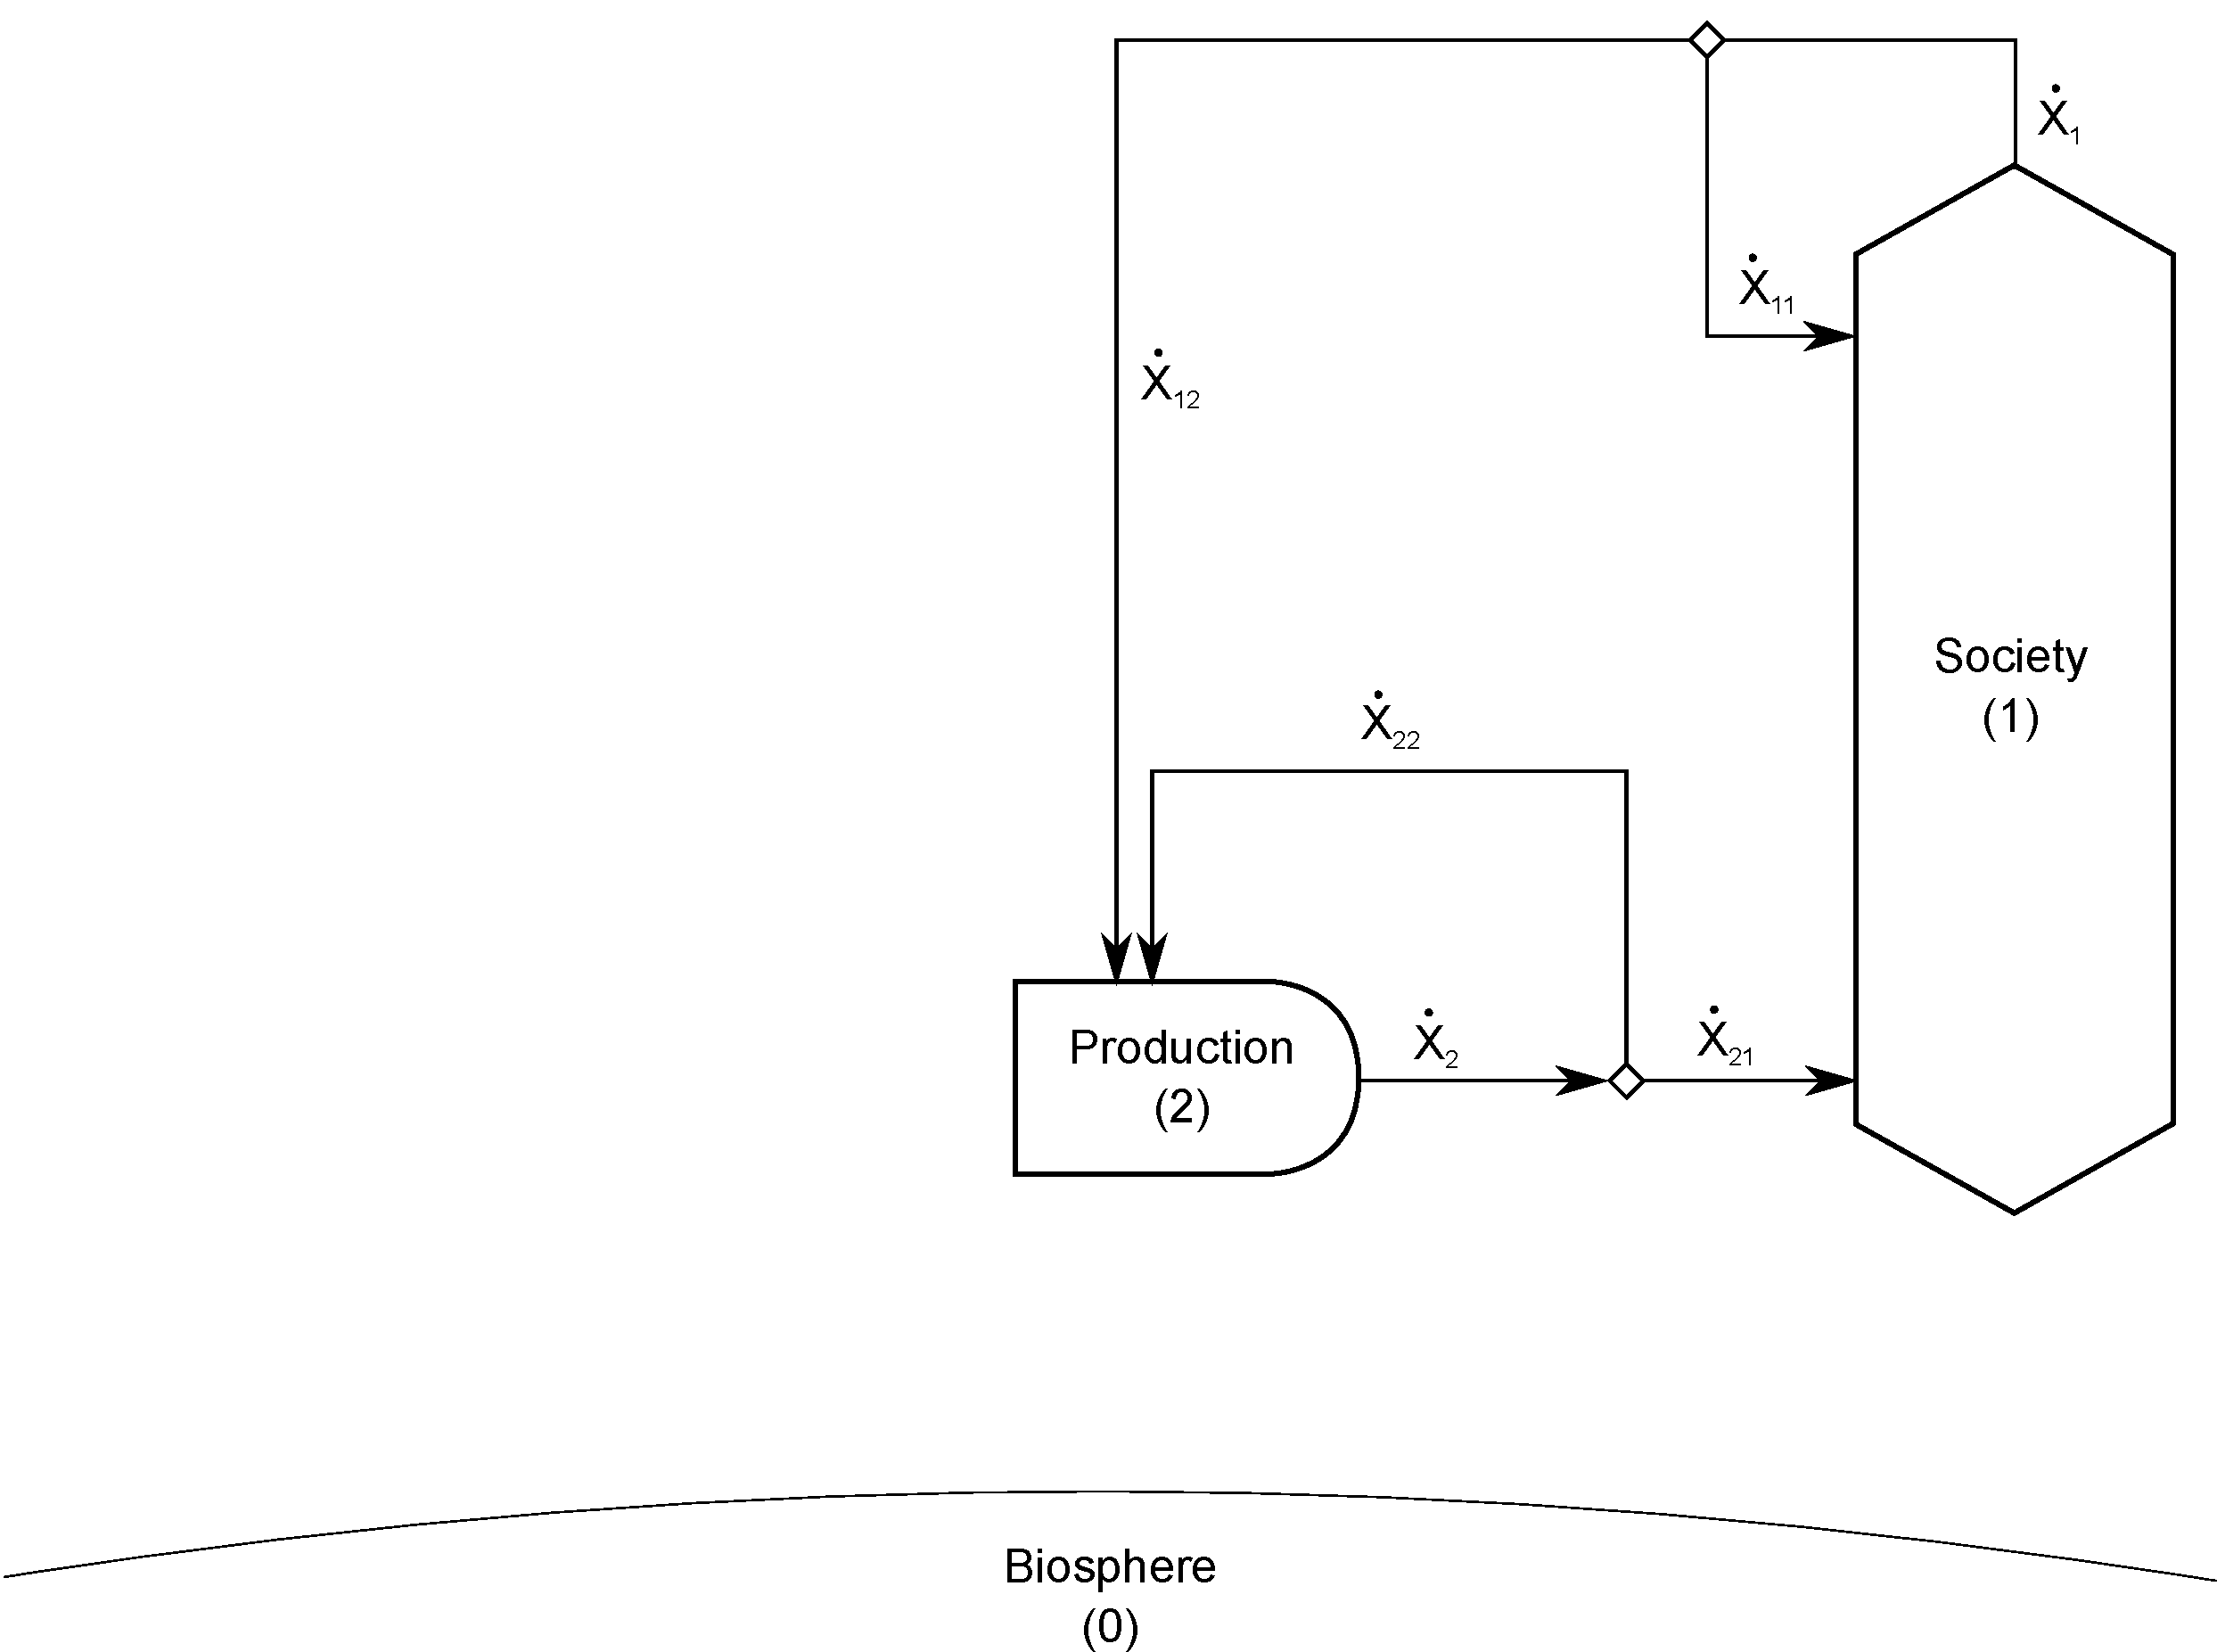
\includegraphics[width=0.8\linewidth]{Part_2/Chapter_Values/images/2_sector_value.pdf}
\caption[Flows of value within a two-sector economy]{Flows of value ($\dot{X}$) within a two-sector economy.}
\label{fig:B_value}
\end{figure}
\end{landscape}

We can account for value flows by writing
the following equations:
%
\begin{equation}\label{eq:B-value-1}
	\frac{\mathrm{d}X_{1}}{\mathrm{d}t}
	= \dot{X}_{11}
	+ \dot{X}_{21}
	- \dot{X}_{1}
	+ \dot{X}_{gen,1}
	- \dot{X}_{dest,1}
\end{equation}
%
and
%
\begin{equation}\label{eq:B-value-2}
	\frac{\mathrm{d}X_{2}}{\mathrm{d}t}
	= \dot{X}_{12}
	+ \dot{X}_{22}
	- \dot{X}_{2}
	+ \dot{X}_{gen,2}
	- \dot{X}_{dest,2}.
\end{equation}

Equations~\ref{eq:B-value-1} and~\ref{eq:B-value-2}
can be generalized as
%
\begin{equation}\label{eq:B-value-generalized}
	\frac{\mathrm{d}X_{j}}{\mathrm{d}t}
	= \sum\limits_{i=1}^n \dot{X}_{ij}
	- \dot{X}_{j}
	+ \dot{X}_{gen,j}
	- \dot{X}_{dest,j},
\end{equation}
%
where $n$ is the number of sectors in the economy, and $j \in [1, n]$.


%%%%%%%%%% Example C: three-sector economy %%%%%%%%%%
\section{Example~C: three-sector economy} % chktex 13
\label{sec:value_example_C}
%%%%%%%%%%

Figure~\ref{fig:C_value} shows flows of value ($\dot{X}$) 
within a three-sector economy. 

\begin{landscape}
\begin{figure}[!ht]
\centering
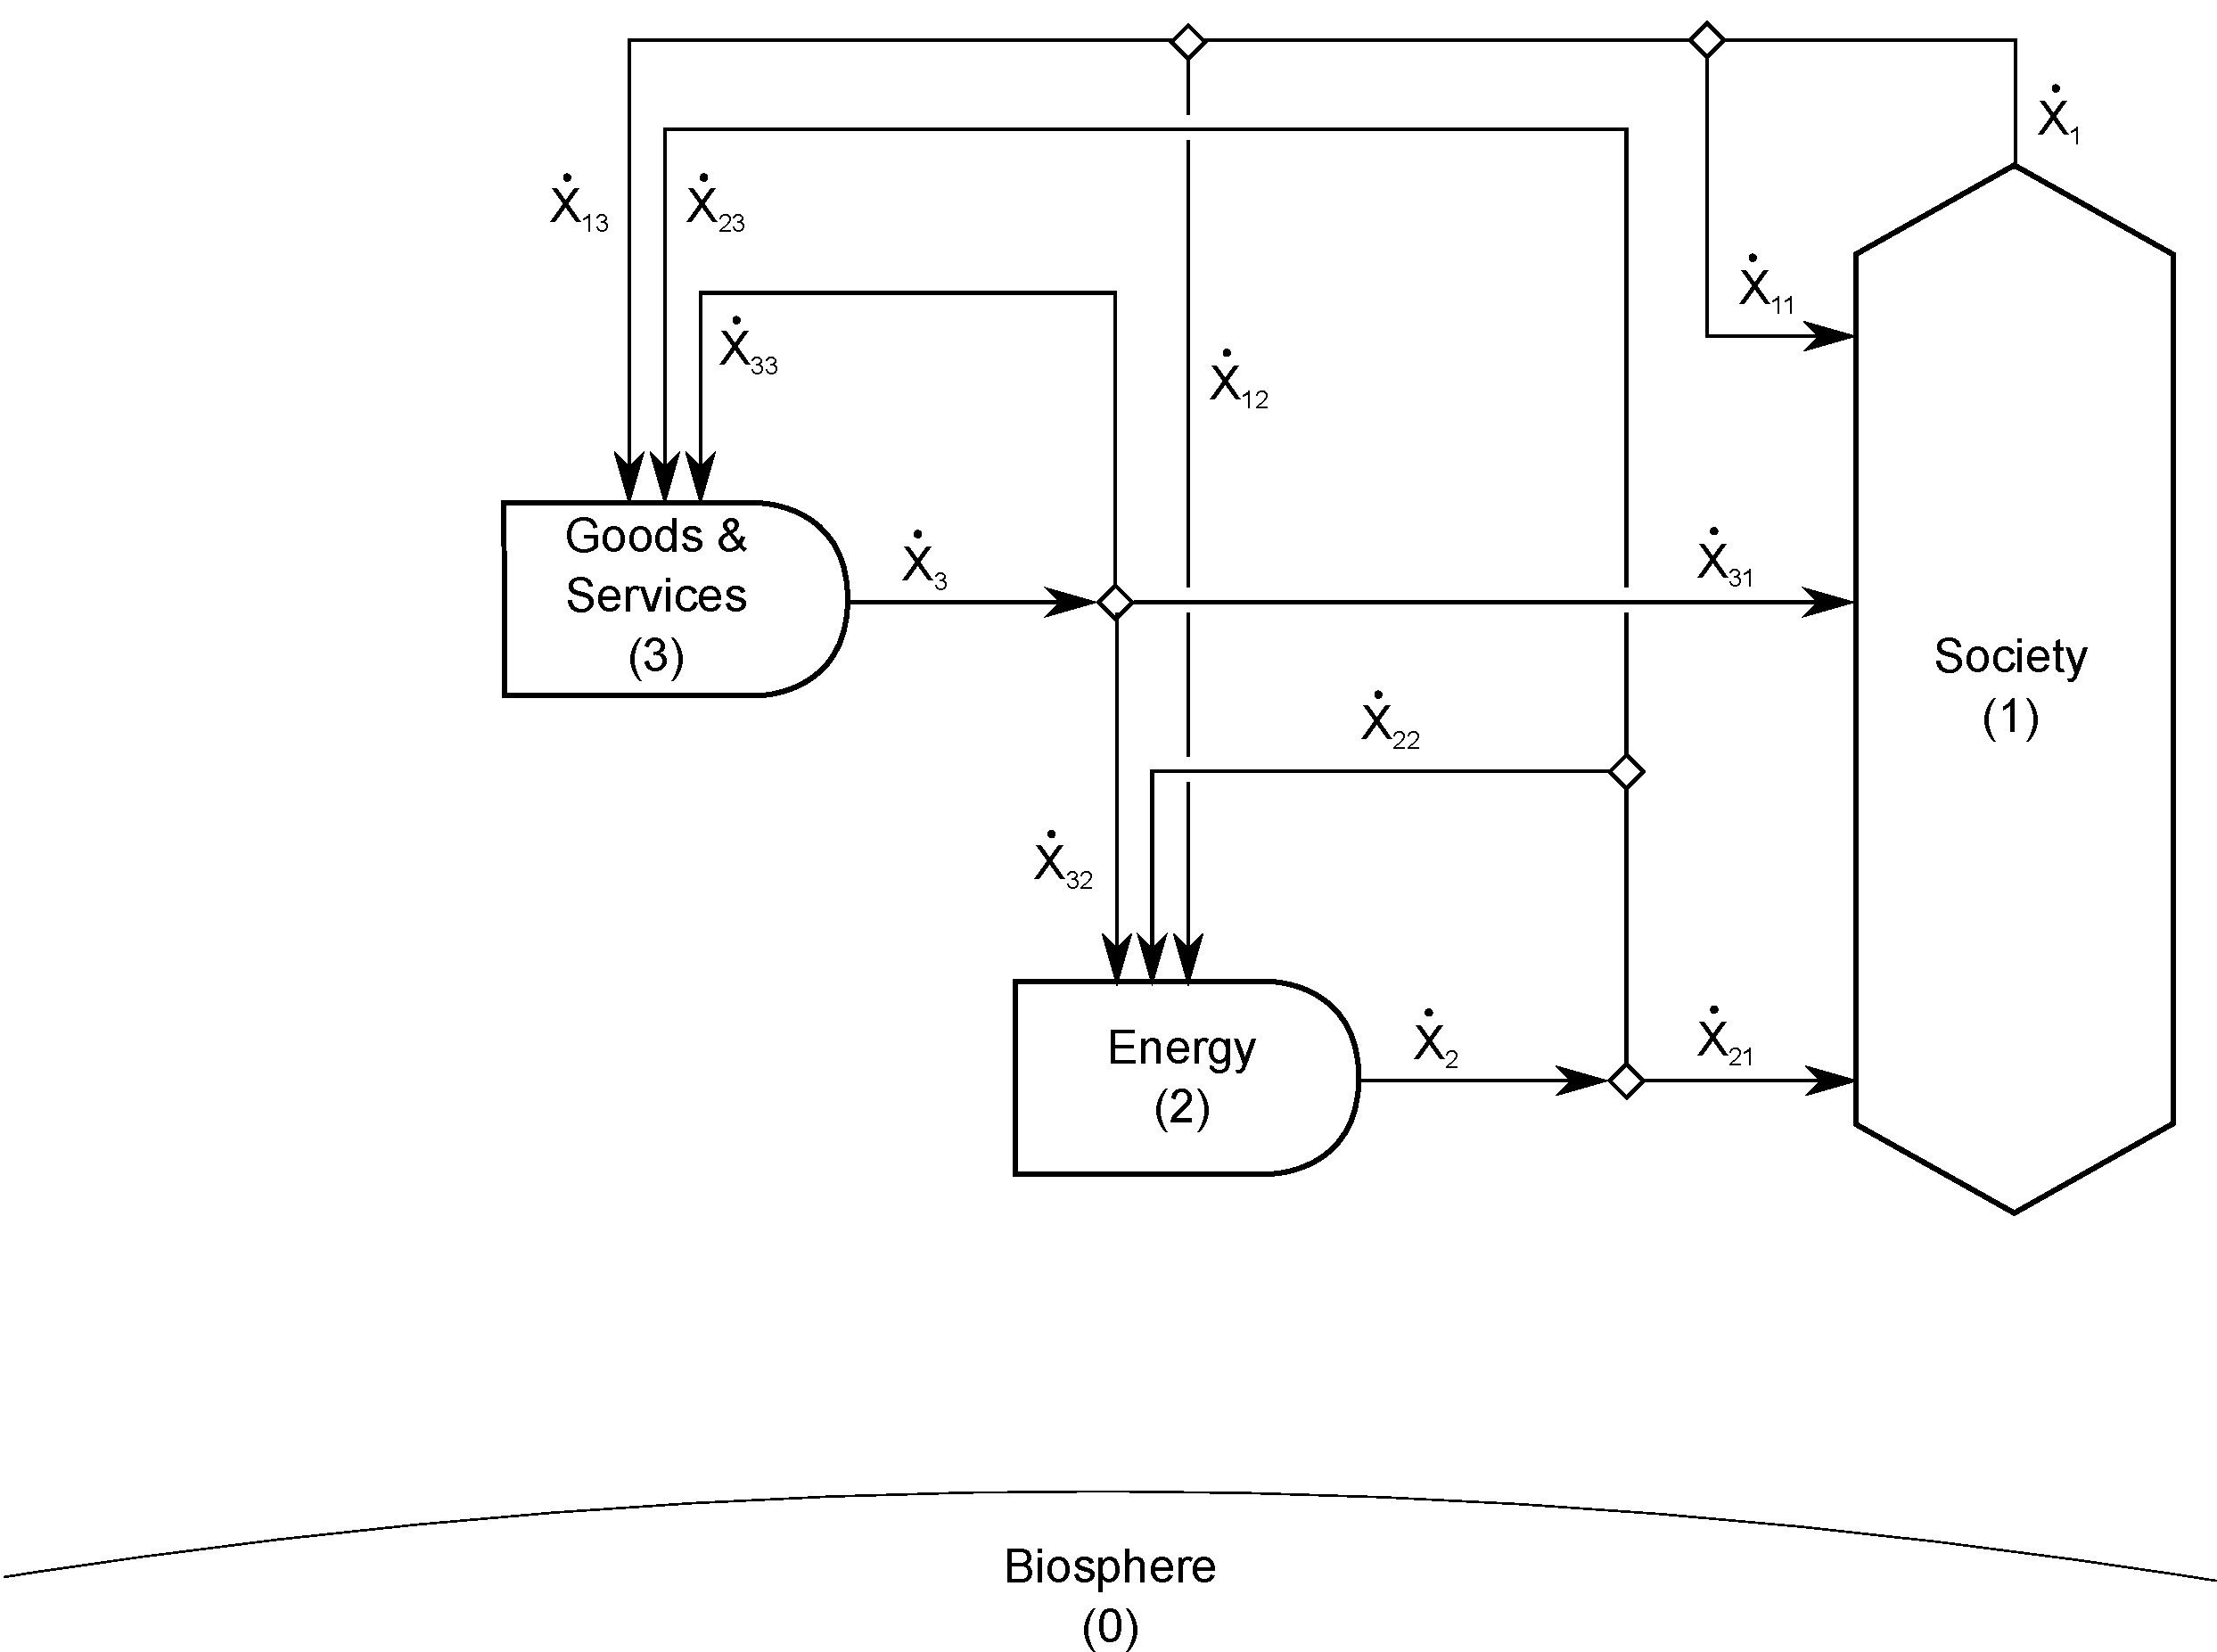
\includegraphics[width=0.8\linewidth]{Part_2/Chapter_Values/images/3_sector_value.pdf}
\caption[Flows of value within a three-sector economy]{Flows of value ($\dot{X}$) within a three-sector economy.}
\label{fig:C_value}
\end{figure}
\end{landscape}

The equations representing flows of value in Example~C are:
%
\begin{equation}\label{eq:C-value-generalized}
	\frac{\mathrm{d}X_{j}}{\mathrm{d}t}
	= \sum\limits_{i=1}^{n} \dot{X}_{ij}
	- \dot{X}_{j}
	+ \dot{X}_{gen,j}
	- \dot{X}_{dest,j},
\end{equation}
%
where $n$ is the number of sectors in the economy, and $j \in [1, n]$.
Equation~\ref{eq:C-value-generalized} is identical to Equation~\ref{eq:B-value-generalized}.
If we sum the value accounting equations for the entire economy, 
we obtain
%
\begin{equation}\label{eq:C-value-economy-a}
	\sum\limits_{j=1}^{n} \frac{\mathrm{d}X_{j}}{\mathrm{d}t}
	= \sum\limits_{j=1}^{n} \sum\limits_{i=1}^{n} \dot{X}_{ij}
	- \sum\limits_{j=1}^{n} \dot{X}_{j}
	+ \sum\limits_{j=1}^{n} \dot{X}_{gen,j}
	- \sum\limits_{j=1}^{n} \dot{X}_{dest,j}.
\end{equation}
%
With the identities
%
\begin{equation} \label{eq:X_identity_1}
	\dot{X}_{j}  
	= \sum\limits_{k=1}^n \dot{X}_{jk}
\end{equation}
%
and
%
\begin{equation} \label{eq:X_identity_2}
	\sum\limits_{j=1}^n\dot{X}_{j}  
	= \sum\limits_{j=1}^n \sum\limits_{k=1}^n \dot{X}_{jk}
	= \sum\limits_{i=1}^n \sum\limits_{k=1}^n \dot{X}_{ik}
	= \sum\limits_{i=1}^n \sum\limits_{j=1}^n \dot{X}_{ij}
	= \sum\limits_{j=1}^n \sum\limits_{i=1}^n \dot{X}_{ij},
\end{equation}
%
Equation~\ref{eq:C-value-economy-a} becomes
%
\begin{equation}\label{eq:C-value-economy-b}
	\sum\limits_{j=1}^{n} \frac{\mathrm{d}X_{j}}{\mathrm{d}t}
	= \sum\limits_{j=1}^{n} \dot{X}_{gen,j}
	- \sum\limits_{j=1}^{n} \dot{X}_{dest,j},
\end{equation}
%
for $j \in [1, n]$, indicating that 
value generation ($\dot{X}_{gen,j}$) 
and destruction ($\dot{X}_{dest,j}$)
are the only mechanisms by which value is accumulated or lost
$\left( \frac{\mathrm{d}X_{j}}{\mathrm{d}t} \right)$
within the economy.  
Equation~\ref{eq:C-value-economy-b} is a mathematical representation of the
value-added approach to measuring GDP\@. The sum of the
value-added across all industries is equivalent to the 
total value of final produced goods.\cite[p.~196]{Landefeld:2008aa}


%%%%%%%%%% Value: Auto industry example %%%%%%%%%%
\section{Value in the US auto industry}
\label{sec:value_auto}
%%%%%%%%%%

To estimate value flows through the automobile industry, 
we use publicly available data from the 
US BEA.%
	\footnote{
	A primer on using the US BEA
	industry data can be found 
	on the BEA website.\cite{Streitwieser:2011aa}
	}
The tables needed to estimate dynamic 
value flows and capital accumulation within the economy 
are primarily the KLEMS%
	\footnote{
	KLEMS is an acronym for 
	capital~(K), labor~(L), energy~(E), materials~(M), and services~(S).
	} 
Intermediate Use
tables and 
the fixed asset, non-residential detail table. 
The KLEMS data tables
are based on the Input-Output (I-O) tables, 
but are at a lower level of aggregation and the inputs are categorized 
into three broad types: energy, materials, and services.

The KLEMS intermediate use data are categorized in the same
way as the input flows in our framework. 
The total material inputs into the auto industry (IOC 3361MV) 
represents the value of resource flows ($\dot{X}_{\dot{R}}$). 
Similarly, the total direct energy inputs into the 
auto industry represents the value of energy flows ($\dot{X}_{\dot{E}}$),
and the total service inputs into the auto industry represents 
short-lived goods ($\dot{X}_{\dot{S}}$).
The fixed asset accounts are
used to estimate capital value flows 
($\dot{X}_{\dot{K}}$) as well as self-use of capital.  
The I-O tables are used to determine gross economic output of the 
auto industry ($\dot{X}_{\dot{P}_{Gross}}$). And subtracting self-use capital and resources
from Gross Economic Output yields Net Economic Output ($\dot{X}_{\dot{P}_{net}}$).

The Capital flow ($\dot{X}_{\dot{K}}$
values are derived from the Fixed Assets tables
provided by the BEA. Two numbers are listed on the figure
 for capital flows because of 
recent changes to the US national accounting methodology
related to Fixed Assets. The first number is the
value for physical capital flows only; the second number (denoted
``w\ R\&D'') is the original number from the Fixed Asset national account, which includes intellectual property. The
difference between the two numbers in the
auto industry is large.

  In 2013, expenditures
related to intellectual property
were categorized as fixed assets and greatly 
increased the monetary value of
capital in national accounts. Because 
our framework is a biophysical approach
to the economy, we subtracted expenditures
Intellectual Property from 
the capital flows derived from the Fixed Asset
table.

Using these data, Figure~\ref{fig:PERKS_value_auto_ind} provides estimates 
of value flows for the US auto industry.
Table~\ref{tab:data} contains a brief summary  
of the data sources that were used 
to obtain the values in Figure~\ref{fig:PERKS_value_auto_ind}. 
Appendix~\ref{chap:auto_value_flows} contains
detailed calculations and sources of data.

The issues surrounding the treatment of capital
in national accounts are captured succinctly
by the
 two numbers for capital flows shown on Figure~\ref{fig:PERKS_value_auto_ind}
 The expansion of the definition of Fixed Assets 
 by the BEA reveals a fundamental shift 
in the US treatment of capital.
 Until the mid-1990s, Fixed Assets included only manufactured, physical assets:
equipment and structures.
In 1996, the BEA expanded the definition to include software. This added
about \$174 billion to the nation's private fixed asset account and 
\$56 billion to the nation's public fixed asset account, less than
1\% of \$23.8 trillion in stock of fixed assets at the time.\cite[p. 20]{BEA2000}

In 2013, the BEA fundamentally revised the definition of Fixed Assets 
to include Research \& Development, as well as production of 
creative works, such as art, music, and television shows. These types of assets,
along with software, were combined together into a 
sub-category in the Fixed Assets account labeled, ``Intellectual Property.''\cite{BEA2013}
The latest  publicly available
fixed assets tables reveal that in 2012  intellectual property accounts for approximately
11\% of the non-residential, private fixed investment (\$3.4
trillion (line 20) out of 
\$32.1 trillion total Private and Government non-residential
fixed assets (line17)). For comparison,
Intellectual Property assets are valued at
more than half the value of all 
manufactured equipment (\$6.6 trillion (line 18)).~\cite{BEA2013Table}

The authors are concerned that the 
 evolution of the definition of capital assets 
is indicative of a great problem. The scarce 
resources available to prepare national
accounts have been allocated toward
 rigorous and time-consuming 
valuation of intangible (albeit valuable) assets, while at the same time 
ignoring any assessment
of the biophysical reality.
This tendency obscures the fact that the the nation may be 
consuming the natural capital on its 
balance sheet. The satellite accounts that once
captured estimates of environmental economic
data were shelved by order of Congress and
replaced by R\&D satellite accounts, which 
were then permanently integrated into national accounts. 
That the BEA has been
forbidden to provide estimates of natural capital,
but was given the mandate to develop a
methodology to value intangible
intellectual property is not comensurate with the work
that should be undertaken in an age of
resource depletion. 




\begin{landscape}
\begin{figure}[!ht]
\centering
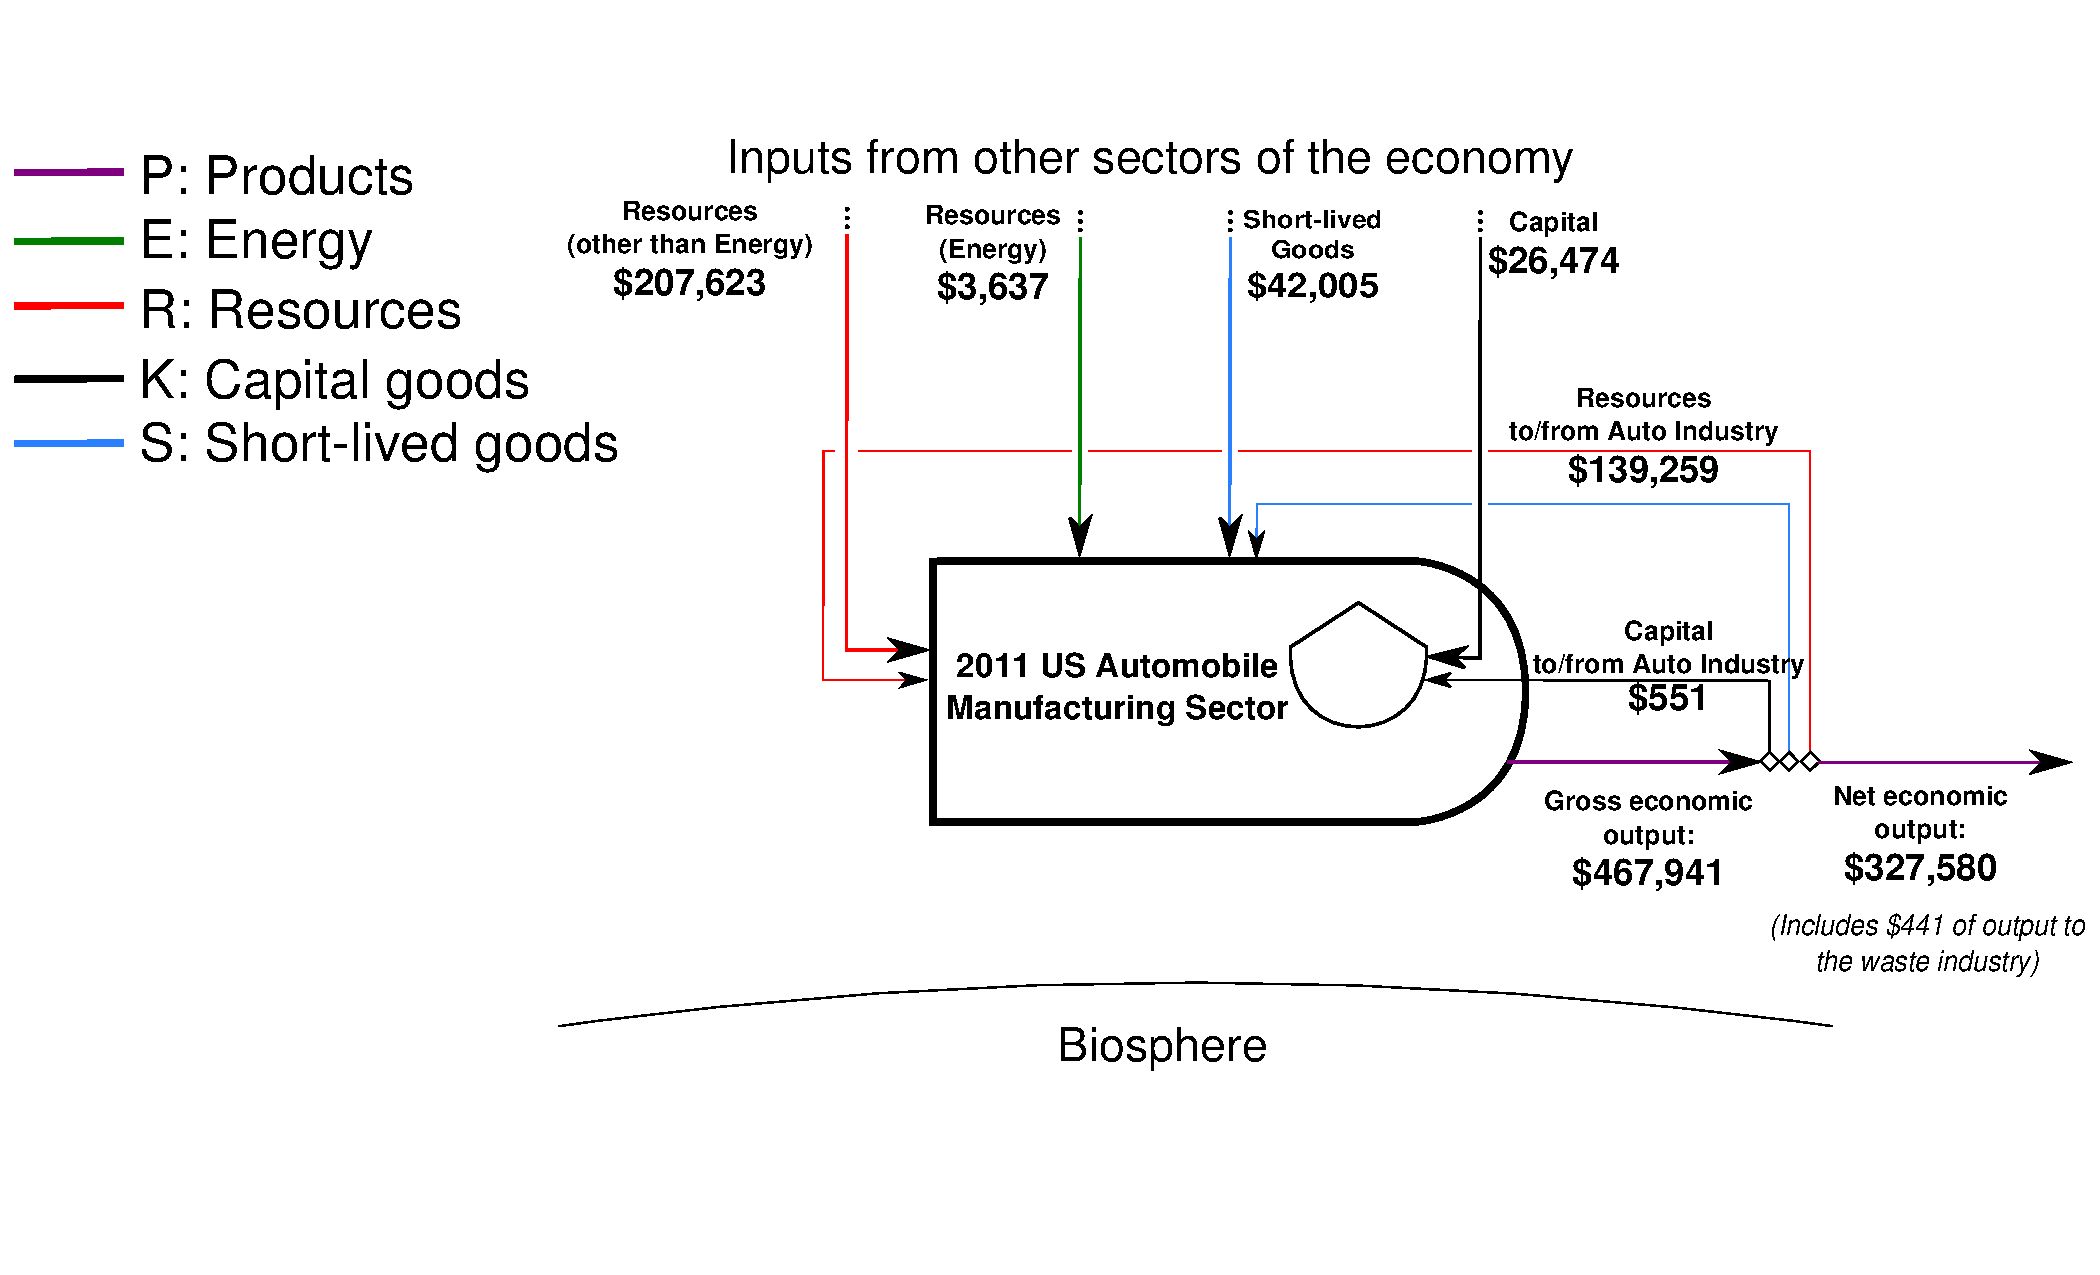
\includegraphics[width=0.8\linewidth]{Part_2/Chapter_Values/images/PERKS_basic_unit_value_auto_ind.pdf}
\caption[Value of material and energy flows 
into and out of the US automobile industry]{Value 
of material and energy flows into and out of the 
US automobile industry (in millions of 2011~US\$).}
\label{fig:PERKS_value_auto_ind}
\end{figure}
\end{landscape}

\begin{table}
\caption[Data Sources for auto industry (IOC 3361MV) example]{Data sources for auto industry (IOC 3361MV) example.}
\begin{center}
  \begin{tabular}{l r @{\hspace{2em}} l}
   \toprule 
     & 2011 USD &   \\ 
Value Flow & (millions) & BEA Data Source \\
	\midrule
    Resources  & \$175,491           & 2011 KLEMS Total Material Inputs \\

   Energy &   3,637&   2011 KLEMS Total Energy Inputs                \\

    Short-lived Goods &   74,578 &   2011 KLEMS Total Services Inputs    \\
%&&\\
    Capital & 14,532  &  2011 Fixed Assets 2011 (non-residential detailed estimates)     \\  

%&&\\
    Gross Economic Output & 482,269  &   2011 Input-Output Use Tables \\

%&&\\
    Resources (self-use)  &  133,961 & 2011 Input-Output Use Tables     \\
%&&\\
    Capital (self-use) & 795 & 2011 Fixed Assets (non-residential detailed estimates)      \\
%&&\\
    Net Economic Output & 333,127   &  Authors' calculations \\
    \bottomrule
  \end{tabular}

\end{center}
\label{tab:data}
\end{table}


%%%%%%%%%% Value: Summary %%%%%%%%%%
\section{Summary}
\label{sec:value_summary}
%%%%%%%%%%

In this chapter, we developed techniques to account for flows of economic value
($\dot{X}$) through economies 
(Section~\ref{sec:Value_Methodology}).
We began with a discussion about theories of value and settled on
the prevailing subjective theory of value for our framework.
Thereafter, value accounting equations were developed and applied to example
economies~A--C % chktex 8
in Sections~\ref{sec:value_example_A}--\ref{sec:value_example_C}. 
We noted the need for terms that describe creation and destruction
of value ($\dot{X}_{gen}$ and $\dot{X}_{dest}$, respectively) 
within economic sectors.
Finally, we explored value flows 
to and from the US auto economy (Section~\ref{sec:value_auto}).

It is important to note at this point that, in contrast to materials and energy,
we found that there is no lack of data on value flows
to and from industry sectors available 
from the US BEA. The value flows
are relatively easily derived from the 
data captured at the point of sale in market transactions. 
However, the US BEA has no values for material and energy flows \emph{to and from the biosphere}.

% Ironically, the data on the physical flows of materials and energy
% to and from the biosphere \emph{are} captured, by
% agencies such as the US Environmental Protection Agency (EPA),
% the US Energy Information Agency (EIA), and the
% International Energy Agency (IEA).
% The challenge for national accounting arises when
% trying to place a value on those flows.
% These challenges were taken up by
% the UN starting in 1991.
% The comprehensive and rigorous UN System of Environmental Economic Accounts (SEEA)
% is now in its third edition,
% and several European Union member states,
% as well as the Phillipines, Canada, and  Austrailia,
% use the SEEA to regularly account value flows to and from the biosphere
% as part of their national accounts.
% However, as recounted in the Prologue, the US BEA has been politically
% prevented from pursuing valuation of material and energy
% flows to and from the biosphere ever since their
% first publication in 1994.

In Chapter~\ref{chap:intensity}, 
we combine results from Chapters~\ref{chap:direct_energy}, 
\ref{chap:embodied_energy}, and~\ref{chap:value}
to develop techniques the estimate the energy intensity
of economic products.


\bibliographystyle{unsrt}
\bibliography{../../Metabolic}



% Always give a unique label
% and use \ref{<label>} for cross-references
% and \cite{<label>} for bibliographic references
% use \sectionmark{}
% to alter or adjust the section heading in the running head
%% Instead of simply listing headings of different levels we recommend to let every heading be followed by at least a short passage of text. Furtheron please use the \LaTeX\ automatism for all your cross-references and citations.

%% Please note that the first line of text that follows a heading is not indented, whereas the first lines of all sequent paragraphs are.

%% Use the standard \verb|equation| environment to typeset your equations, e.g.
%
%% \begin{equation}
%% a \times b = c\;,
%% \end{equation}
%
%% however, for multiline equations we recommend to use the \verb|eqnarray|
%% environment\footnote{In physics texts please activate the class option \texttt{vecphys} to depict your vectors in \textbf{\itshape boldface-italic} type - as is customary for a wide range of physical jects.}.
%% \begin{eqnarray}
%% a \times b = c \nonumber\\
%% \vec{a} \cdot \vec{b}=\vec{c}
%% \label{eq:01}
%% \end{eqnarray}

%% \section{section Heading}
%% \label{sec:2}
%% Instead of simply listing headings of different levels we recommend to let every heading be followed by at least a short passage of text. Furtheron please use the \LaTeX\ automatism for all your cross-references\index{cross-references} and citations\index{citations} as has already been described in Sect.~\ref{sec:2}.

%% \begin{quotation}
%% Please do not use quotation marks when quoting texts! Simply use the \verb|quotation| environment -- it will automatically render Springer's preferred layout.
%% \end{quotation}


%% \section{section Heading}
%% Instead of simply listing headings of different levels we recommend to let every heading be followed by at least a short passage of text. Furtheron please use the \LaTeX\ automatism for all your cross-references and citations as has already been described in Sect.~\ref{sec:2}, see also Fig.~\ref{fig:1}\footnote{If you copy text passages, figures, or tables from other works, you must obtain \textit{permission} from the copyright holder (usually the original publisher). Please enclose the signed permission with the manucript. The sources\index{permission to print} must be acknowledged either in the captions, as footnotes or in a separate section of the book.}

%% Please note that the first line of text that follows a heading is not indented, whereas the first lines of all sequent paragraphs are.

% For figures use
%
%% \begin{figure}[b]
%% \sidecaption
% Use the relevant command for your figure-insertion program
% to insert the figure file.
% For example, with the option graphics use
%% \includegraphics[scale=.65]{figure}
%
% If not, use
%\picplace{5cm}{2cm} % Give the correct figure height and width in cm
%
%% \caption{If the width of the figure is less than 7.8 cm use the \texttt{sidecapion} command to flush the caption on the left side of the page. If the figure is positioned at the top of the page, align the sidecaption with the top of the figure -- to achieve this you simply need to use the optional argument \texttt{[t]} with the \texttt{sidecaption} command}
%% \label{fig:1}       % Give a unique label
%% \end{figure}


%% \paragraph{Paragraph Heading} %
%% Instead of simply listing headings of different levels we recommend to let every heading be followed by at least a short passage of text. Furtheron please use the \LaTeX\ automatism for all your cross-references and citations as has already been described in Sect.~\ref{sec:2}.

%% Please note that the first line of text that follows a heading is not indented, whereas the first lines of all sequent paragraphs are.

%% For typesetting numbered lists we recommend to use the \verb|enumerate| environment -- it will automatically render Springer's preferred layout.

%% \begin{enumerate}
%% \item{Livelihood and survival mobility are oftentimes coutcomes of uneven socioeconomic development.}
%% \begin{enumerate}
%% \item{Livelihood and survival mobility are oftentimes coutcomes of uneven socioeconomic development.}
%% \item{Livelihood and survival mobility are oftentimes coutcomes of uneven socioeconomic development.}
%% \end{enumerate}
%% \item{Livelihood and survival mobility are oftentimes coutcomes of uneven socioeconomic development.}
%% \end{enumerate}


%% \paragraph{paragraph Heading} In order to avoid simply listing headings of different levels we recommend to let every heading be followed by at least a short passage of text. Use the \LaTeX\ automatism for all your cross-references and citations as has already been described in Sect.~\ref{sec:2}, see also Fig.~\ref{fig:2}.

%% Please note that the first line of text that follows a heading is not indented, whereas the first lines of all sequent paragraphs are.

%% For unnumbered list we recommend to use the \verb|itemize| environment -- it will automatically render Springer's preferred layout.

%% \begin{itemize}
%% \item{Livelihood and survival mobility are oftentimes coutcomes of uneven socioeconomic development, cf. Table~\ref{tab:1}.}
%% \begin{itemize}
%% \item{Livelihood and survival mobility are oftentimes coutcomes of uneven socioeconomic development.}
%% \item{Livelihood and survival mobility are oftentimes coutcomes of uneven socioeconomic development.}
%% \end{itemize}
%% \item{Livelihood and survival mobility are oftentimes coutcomes of uneven socioeconomic development.}
%% \end{itemize}

%% \begin{figure}[t]
%% \sidecaption[t]
% Use the relevant command for your figure-insertion program
% to insert the figure file.
% For example, with the option graphics use
%% \includegraphics[scale=.65]{figure}
%
% If not, use
%\picplace{5cm}{2cm} % Give the correct figure height and width in cm
%
%% \caption{Please write your figure caption here}
%% \label{fig:2}       % Give a unique label
%% \end{figure}

%% \runinhead{Run-in Heading Boldface Version} Use the \LaTeX\ automatism for all your cross-references and citations as has already been described in Sect.~\ref{sec:2}.

%% \runinhead{Run-in Heading Italic Version} Use the \LaTeX\ automatism for all your cross-refer\-ences and citations as has already been described in Sect.~\ref{sec:2}\index{paragraph}.
% Use the \index{} command to code your index words
%
% For tables use
%
%% \begin{table}
%% \caption{Please write your table caption here}
%% \label{tab:1}       % Give a unique label
%
% For LaTeX tables use
%
%% \begin{tabular}{p{2cm}p{2.4cm}p{2cm}p{4.9cm}}
%% \hline\noalign{\smallskip}
%% Classes & class & Length & Action Mechanism  \\
%% \noalign{\smallskip}\svhline\noalign{\smallskip}
%% Translation & mRNA$^a$  & 22 (19--25) & Translation repression, mRNA cleavage\\
%% Translation & mRNA cleavage & 21 & mRNA cleavage\\
%% Translation & mRNA  & 21--22 & mRNA cleavage\\
%%Translation & mRNA  & 24--26 & Histone and DNA Modification\\
%%\noalign{\smallskip}\hline\noalign{\smallskip}
%%\end{tabular}
%%$^a$ Table foot note (with superscript)
%%\end{table}
%
%% \section{Section Heading}
%%\label{sec:3}
% Always give a unique label
% and use \ref{<label>} for cross-references
% and \cite{<label>} for bibliographic references
% use \sectionmark{}
% to alter or adjust the section heading in the running head
%% Instead of simply listing headings of different levels we recommend to let every heading be followed by at least a short passage of text. Furtheron please use the \LaTeX\ automatism for all your cross-references and citations as has already been described in Sect.~\ref{sec:2}.

%% Please note that the first line of text that follows a heading is not indented, whereas the first lines of all sequent paragraphs are.

%%If you want to list definitions or the like we recommend to use the Springer-enhanced \verb|description| environment -- it will automatically render Springer's preferred layout.

%%\begin{description}[Type 1]
%%\item[Type 1]{That addresses central themes pertainng to migration, health, and disease. In Sect.~\ref{sec:1}, Wilson discusses the role of human migration in infectious disease distributions and patterns.}
%%\item[Type 2]{That addresses central themes pertainng to migration, health, and disease. In Sect.~\ref{sec:2}, Wilson discusses the role of human migration in infectious disease distributions and patterns.}
%%\end{description}

%%\section{section Heading} %
%% In order to avoid simply listing headings of different levels we recommend to let every heading be followed by at least a short passage of text. Use the \LaTeX\ automatism for all your cross-references and citations citations as has already been described in Sect.~\ref{sec:2}.

%% Please note that the first line of text that follows a heading is not indented, whereas the first lines of all sequent paragraphs are.

%% \begin{svgraybox}
%% If you want to emphasize complete paragraphs of texts we recommend to use the newly defined Springer class option \verb|graybox| and the newly defined environment \verb|svgraybox|. This will produce a 15 percent screened box 'behind' your text.

%% If you want to emphasize complete paragraphs of texts we recommend to use the newly defined Springer class option and environment \verb|svgraybox|. This will produce a 15 percent screened box 'behind' your text.
%% \end{svgraybox}


%% \section{section Heading}
%%Instead of simply listing headings of different levels we recommend to let every heading be followed by at least a short passage of text. Furtheron please use the \LaTeX\ automatism for all your cross-references and citations as has already been described in Sect.~\ref{sec:2}.

%% Please note that the first line of text that follows a heading is not indented, whereas the first lines of all sequent paragraphs are.

%% \begin{theorem}
%% Theorem text goes here.
%% \end{theorem}
%
% or
%
%% \begin{definition}
%% Definition text goes here.
%% \end{definition}

%% \begin{proof}
%\smartqed
%% Proof text goes here.
%% \qed
%% \end{proof}

%%\paragraph{Paragraph Heading} %
%% Instead of simply listing headings of different levels we recommend to let every heading be followed by at least a short passage of text. Furtheron please use the \LaTeX\ automatism for all your cross-references and citations as has already been described in Sect.~\ref{sec:2}.

%% Note that the first line of text that follows a heading is not indented, whereas the first lines of all subsequent paragraphs are.
%
% For built-in environments use
%
%%\begin{theorem}
%%Theorem text goes here.
%%\end{theorem}
%
%%\begin{definition}
%%Definition text goes here.
%%\end{definition}
%
%%\begin{proof}
%%\smartqed
%% Proof text goes here.
%%\qed
%%\end{proof}
%
%% \begin{acknowledgement}
%% If you want to include acknowledgments of assistance and the like at the end of an individual chapter please use the \verb|acknowledgement| environment -- it will automatically render Springer's preferred layout.
%% \end{acknowledgement}
%
%% \section*{Appendix}
%% \addcontentsline{toc}{section}{Appendix}
%
%% When placed at the end of a chapter or contribution (as opposed to at the end of the book), the numbering of tables, figures, and equations in the appendix section continues on from that in the main text. Hence please \textit{do not} use the \verb|appendix| command when writing an appendix at the end of your chapter or contribution. If there is only one the appendix is designated ``Appendix'', or ``Appendix 1'', or ``Appendix 2'', etc. if there is more than one.

%% \begin{equation}
%% a \times b = c
%% \end{equation}
% Problems or Exercises should be sorted chapterwise
%% \section*{Problems}
%% \addcontentsline{toc}{section}{Problems}
%
% Use the following environment.
% Don't forget to label each problem;
% the label is needed for the solutions' environment
%% \begin{prob}
%% \label{prob1}
%% A given problem or Excercise is described here. The
%% problem is described here. The problem is described here.
%% \end{prob}

%% \begin{prob}
%% \label{prob2}
%% \textbf{Problem Heading}\\
%% (a) The first part of the problem is described here.\\
%% (b) The second part of the problem is described here.
%% \end{prob}


